% !TEX root = C:/Users/piyus/knowledge/Project_Specific_Knowledge/public/fm_radio/stages/variable_gain_amp/variable_gain_amp.tex
\documentclass[12pt, letterpaper]{article}

\usepackage{hyperref}
\usepackage{graphicx}
\graphicspath{ {C:/Users/piyus/knowledge/Project_Specific_Knowledge/public/fm_radio/stages/variable_gain_amp/pictures} }

\title{Variable Gain Amplifier Notes}
\author{Piyush Sud}
\date{10/13/2024}
\begin{document}
\maketitle

\pagebreak

\section{High Level Design}

\begin{itemize}
    \item what range of amplitudes are we looking for?
    \item Based on this: \url{https://forum.allaboutcircuits.com/threads/voltage-on-an-antenna.88982/}
    \item It seems like FM receiver gain is on the order of 100 - 120 dB and the input is typically in the high uV to low mV range.
    \item According to \url{https://electronics.stackexchange.com/questions/28404/what-is-the-voltage-range-of-a-standard-headphone-jack-from-a-phone}, it seems like a sufficient power for headphones is around 5 mW. Have confirmed this from other googling as well. Given that my headphones have an impedance of 38 ohms, \(0.005 = V^2/38 => V = 0.436V\). 
    \item According to this link, the coupling coefficient of a foster seeley discriminator can be as low as 0.1, and a good value considering the tradeoff between sensitivity vs. linearity is k = 0.3. 
    \item \url{https://www.academia.edu/50833927/What_simulation_of_the_Foster_Seeley_discriminator_can_reveal?sm=b}. This link also provides a lot of simulation data!
    \item Assuming the antenna provides a signal of amplitude of 1 mV, a coupling coefficient of 0.3, assuming minimal loss in the right half of the discriminator, and a voltage of 0.436V, we need a voltage gain of ~1.45k = 63.2273600447 dB. 
    \item The MAR-8ASM+ has a gain of 31.5 dB at 0.1 GHz, and I'm assuming it's similar for the IF. This gives us 31.5*2 = 63 dB, which is almost exactly what we need. 
    \item We need another amplifier with adjustable gain to set the gain to the appropriate value for headphones.
    \item This seems like a good variable gain amplifier: https://www.digikey.com/en/products/detail/texas-instruments/VCA824IDGST/1766828?s=N4IgTCBcDaIGoGECCAOMAWAkgEQOIGUAVEAXQF8g
    \item Bandwidth if 320 MHz, which is much higher than what we need
    \item Gain can be adjusted from 2 to 40 V/V.
    \item We should just use that for the IF amplifier as well, since the gain can also be too high, as in some cases, it can go up the 10s or 100s of mV range: https://www.quora.com/How-many-mV-should-I-expect-from-an-AM-FM-radio-antenna
\end{itemize}

\section{Detailed Design}

\begin{itemize}
    \item RF/RG = 40V/V as the maximum. Note that the gain isn't perfectly linear, so RF/RG doesn't exactly give you the gain. However, since we can adjust the gain with a potentiometer, this doesn't really matter.
    \item If we choose a gain of 20 dB = 10V/V for the IF, then to achieve a nominal gain of 63.23 dB mentioned above, we'd need 11.73 dB of amplification in the last stage = 3.86V/V. 
    \item For some reason (probably because it creates a pole, reducing the BW), they used small resistor values for Rf and Rg in their example circuits, so let's do the same. For the gain of 10V/V for the IF, let's choose Rf = 500 and Rg = 50. For the gain of 3.86V/V, we need a nominal Rf = 500 and Rg = 129. Let's say that we want the gain to be able to up to 40 V/V, then we need Rg to go down to 12.5. If we want the gain to down to 2V/V, then we need Rg = 250. Therefore the pot range we are looking for is [12.5, 250]. The bottom value in the range should be easy to achieve since most pots can typically go down to 1 to 2 percent of their max value. 
    \item It seems like a resistor between the feedback pin and the input is only used if we need the output voltage to be both a function of Vg and Vin. However, in this case, we only really need it to be a function of Vin since we can set Rf/Rg using a potentiometer, and the output voltage is also proportional to Rf/Rg.
    \item The input impedance is high impedance, so we can just put a 50 ohm resistor to ground.
    \item The output also needs a 50 ohm output resistor in series. 
    \item We can use the following circuit from the datasheet: 
    \begin{figure}[h]
        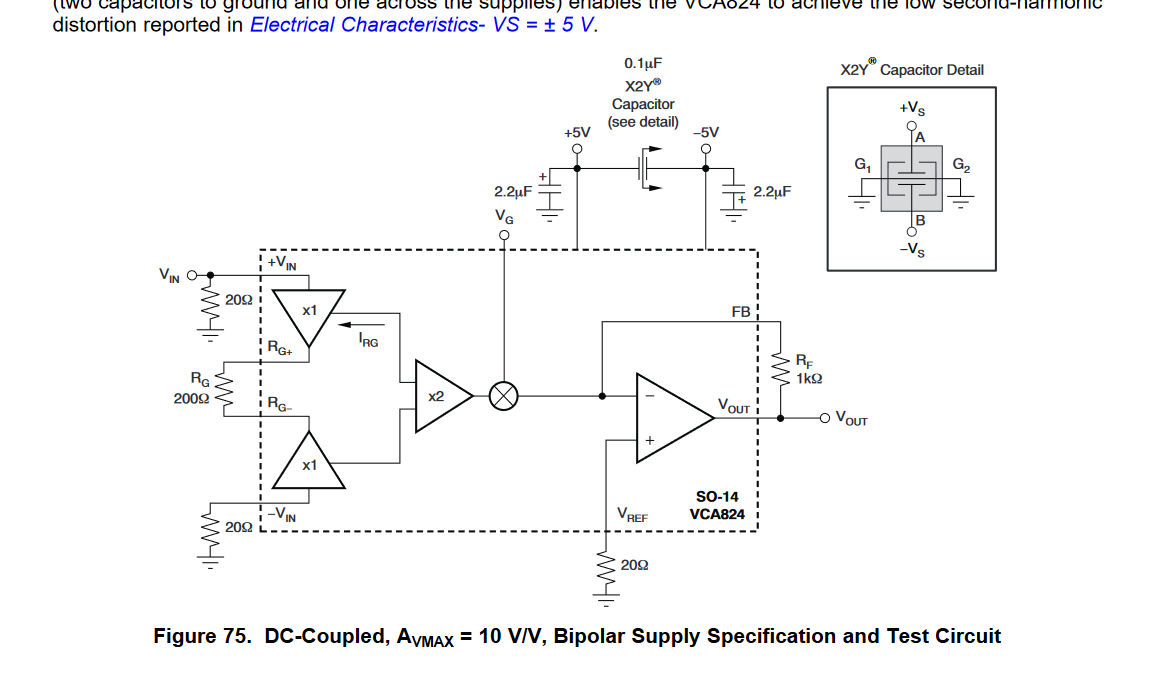
\includegraphics[width=\textwidth]{application_circuit}
    \end{figure}
\end{itemize}

\end{document}
